\addtocontents{xms}{\protect\addvspace{10pt}}

\chapter{Càlculs Bàsics}\label{sec:ch-calc-bas}

\section{Introducció}
Es tracten en aquest capítol càlculs bàsics que poden utilitzar-se en la
resolució de diversos problemes electrotècnics.



\section{Càlculs en tant per u} \label{sec:seccio_pu} \index{pu}\index{tant per u}

Les magnituds expressades en tant per u (també: en tant per unitat, o en per unitat) són útils quan es treballa
amb xarxes de corrent altern on hi ha transformadors, i, per tant, més d'un nivell de tensió. S'acostuma a afegir el símbol «pu» a una magnitud expressada en tant per u,  per fer explícit aquest fet ---tal com s'afegeix el símbol «\%» a una magnitud expressada en tant per cent.

\subsection{Mètode de càlcul} \index{pu!mètode de càlcul}

\index{pu!magnituds base fonamentals} El primer pas consisteix a
escollir unes magnituds base. Les magnituds base fonamentals són la
potència i la tensió; s'escull una potència base $S\ped{B}$ per a
tota la xarxa, i tantes tensions base $U_{\text{B}_1}, U_{\text{B}_2}, \ldots,
U_{\text{B}_n}$ com nivells de tensió
diferents tingui la xarxa:
\begin{equation}
   \text{Magnituds base fonamentals:}\;\left\{
\begin{array}{l}
   S\ped{B} \\
   U_{\text{B}_1}, U_{\text{B}_2}, \ldots, U_{\text{B}_n}
\end{array}
\right.
\end{equation}

Normalment, s'escull com a tensions base les tensions nominals dels transformadors de la
xarxa, i com a potència base la potència nominal d'un dels transformadors o generadors de la xarxa; també és usual utilitzar com a potència base el valor \qty{100}{MVA}.

En el cas de circuits monofàsics, les tensions base són les tensions monofàsiques, o fase-neutre $U\ped{FN}$, i la potència base és la potència monofàsica $S\ped{1F}$. En el cas de circuits trifàsics, podem escollir com a tensions base les tensions fase-neutre $U\ped{FN}$ i com a potència base la potència  monofàsica $S\ped{1F}$, o bé podem escollir com a tensions base les tensions fase-fase $U\ped{FF}$ i com a potència base la potència trifàsica $S\ped{3F}$.

\index{pu!magnituds base}A partir de la potència base i de les tensions base es
defineixen els corrents base $I_{\text{B}_i}$, les impedàncies base $Z_{\text{B}_i}$ i les
admitàncies base $Y_{\text{B}_i}$. Segons que s'utilitzin les tensions i potències monofàsiques o trifàsiques com a magnituds base, tenim:
\begin{equation}
\begin{array}{c}  S\ped{B}=S\ped{1F} \\ U_{\text{B}_i} = U_{\text{FN}_i} \\ (i=1,\ldots,n) \end{array}
\left\{
\begin{array}{l}
   I_{\text{B}_i} = \dfrac{S\ped{B}}{U_{\text{B}_i}} \\[2.5ex]
   Z_{\text{B}_i} = \dfrac{U_{\text{B}_i}^2}{S\ped{B}} = \dfrac{U_{\text{B}_i}}{I_{\text{B}_i}} \\[2.5ex]
   Y_{\text{B}_i} = \dfrac{S\ped{B}}{U_{\text{B}_i}^2} = \dfrac{I_{\text{B}_i}}{U_{\text{B}_i}}
\end{array}
\right.
\qquad\qquad
\begin{array}{c} S\ped{B}=S\ped{3F} \\ U_{\text{B}_i} = U_{\text{FF}_i} \\ (i=1,\ldots,n) \end{array}
\left\{
\begin{array}{l}
   I_{\text{B}_i} = \dfrac{S\ped{B}}{\sqrt{3} U_{\text{B}_i}} \\[2.5ex]
   Z_{\text{B}_i} = \dfrac{U_{\text{B}_i}^2}{S\ped{B}}= \dfrac{U_{\text{B}_i}}{\sqrt{3} I_{\text{B}_i}} \\[2.5ex]
   Y_{\text{B}_i} = \dfrac{S\ped{B}}{U_{\text{B}_i}^2} = \dfrac{\sqrt{3} I_{\text{B}_i}}{U_{\text{B}_i}}
\end{array}
\right.
\label{eq:bases_pu}
\end{equation}

Les magnituds expressades en tant per u ---escrites usualment amb minúscules--- s'obtenen
dividint les magnituds reals ---escrites usualment amb majúscules--- pels valors base corresponents:
\begin{equation}
   \cmplx{s} = \frac{\cmplx{S}}{S\ped{B}} \qquad \cmplx{u} = \frac{\cmplx{U}}{U\ped{B}} \qquad \cmplx{i} = \frac{\cmplx{I}}{I\ped{B}} \qquad \cmplx{z} = \frac{\cmplx{Z}}{Z\ped{B}} \qquad \cmplx{y} = \frac{\cmplx{Y}}{Y\ped{B}}
\end{equation}

Quan es tracta de resoldre circuits trifàsics equilibrats fem servir sempre els circuits equivalents per fase, i podem escollir aleshores com a valors base per a la potència i la tensió, la potència monofàsica $S\ped{1F}$ i la tensió fase-neutre $U\ped{FN}$ respectivament, o la potència trifàsica $S\ped{3F}$ i la tensió fase-fase $U\ped{FF}$ respectivament.


 Quan fem la reducció dels valors reals als valors en tant per u, hem de ser conseqüents i utilitzar sempre les potències monofàsiques i les tensions fase-neutre, o fer servir sempre les potències trifàsiques i les tensions fase-fase.

 Com que es verifica $S\ped{3F}=3 S\ped{1F}$ i $U\ped{FF}=\sqrt{3}U\ped{FN}$, els valors  del corrent base $I\ped{B}$, de la impedància base $Z\ped{B}$ i  de l'admitància base $Y\ped{B}$ són els mateixos, tant si utilitzem $S\ped{B}=S\ped{1F}$ i $U\ped{B}=U\ped{FN}$, com si utilitzem $S\ped{B}=S\ped{3F}$ i $U\ped{B}=U\ped{FF}$.

 En ambdós casos $I\ped{B}$ i $\cmplx{I}$ són corrents fase-neutre, $Z\ped{B}$ i $\cmplx{Z}$ són impedàncies  fase-neutre i $Y\ped{B}$ i $\cmplx{Y}$ són admitàncies fase-neutre; si tenim càrregues connectades en triangle, caldrà transformar-les en càrregues equivalents connectades en estrella per tal de poder aplicar aquest mètode (vegeu la secció \ref{secc:d_y}).

El pas següent consisteix a representar el circuit equivalent en tant
per u, i resoldre'l; en el cas de circuits trifàsics, i a causa del procés utilitzat, el circuit equivalent en tant per u esdevé un circuit monofàsic, i com a tal l'hem de resoldre, és a dir, sense la intervenció del factor $\sqrt{3}$.

Un cop resolt el circuit, es multipliquen les magnituds obtingudes en tant per u, pels
seus valors base respectius, per tal d'obtenir les magnituds reals:
\begin{equation}
   \cmplx{S} = \cmplx{s} S\ped{B} \qquad \cmplx{U} = \cmplx{u} U\ped{B} \qquad \cmplx{I} = \cmplx{i} I\ped{B} \qquad \cmplx{Z} = \cmplx{z} Z\ped{B} \qquad \cmplx{Y} = \cmplx{y} Y\ped{B}
\end{equation}

\subsection{Canvi de base}\label{sec:canvi-base} \index{pu!canvi de base}

Normalment, les impedàncies dels transformadors ---impedància de curtcircuit--- o dels generadors ---impedància sincrònica, transitòria, etc.--- estan referides a les magnituds nominals de la màquina en qüestió.


Si les magnituds base escollides coincideixen amb les nominals de la màquina,
la impedància de la màquina en qüestió estarà expressada ja directament en tant per u, respecte d'aquesta base.

 En canvi, si les magnituds base són diferents de les nominals de la màquina, caldrà fer un canvi de base per tal de referir la impedància de la màquina a les magnituds base escollides.

De forma genèrica, si $\cmplx{z}$ és una impedància referida a la base $Z\ped{B}$, $U\ped{B}$ i $S\ped{B}$, podem obtenir la impedància $\cmplx{z}'$ referida a la base $Z_{\text{B}'}$, $U_{\text{B}'}$ i $S_{\text{B}'}$, mitjançant el canvi:
\begin{equation}
   \cmplx{z}' = \cmplx{z} \; \frac{Z\ped{B}}{Z_{\text{B}'}} = \cmplx{z} \; \frac{U\ped{B}^2}{U_{\text{B}'}^2} \; \frac{S_{\text{B}'}}{S\ped{B}}\label{eq_pu_canvi_base}
\end{equation}


\begin{exemple}[\MetodeCalculPU{}]\label{ex:MetodeCalculPU}
	\addcontentsxms{\MetodeCalculPU}
    Es tracta de calcular el corrent de curtcircuit trifàsic en el punt F de la xarxa següent, suposant
    que el sistema està treballant en buit.
    \begin{center}
        \input{Imatges/Cap-CalcBas-pu-Circuit1.pdf_tex}
    \end{center}

    Les dades del generador G, del transformador T1, de la línia L i del transformador T2 són:
    \begin{align*}
       S\ped{G} &= \qty{60}{MVA} & S\ped{T1} &= \qty{40}{MVA} & l\ped{L} &= \qty{22}{km} & S\ped{T2} &=
       \qty{12}{MVA} \\
       U\ped{G} &= \qty{10,5}{kV} & m\ped{T1} &= \qty{10,5}{kV}\!:\!\qty{63}{kV} & U\ped{L} &= \qty{60}{kV} & m\ped{T2} &= \qty{60}{kV}\!:\!\qty{10,5}{kV} \\
       X''\ped{G} &= \qty{12}{\percent} & X\ped{T1} &= \qty{10}{\percent} & X\ped{L} &= \qty{0,4}{\ohm/km} & X\ped{T2} &= \qty{8}{\percent}
    \end{align*}

    Escollim, en primer lloc, les següents magnituds base: $S\ped{B} = \qty{60}{MVA}$ i $U\ped{B}
    = \qty{10,5}{kV} / \qty{63}{kV} / \qty{10,5}{kV}$.

    Calculem a continuació els valors en tant per u, dels diferents elements de la xarxa:

    \textbf{Generador}. En coincidir les magnituds base amb les nominals del generador tenim
     directament:
    \[
    x''\ped{G} = \qty{0,12}{pu}
    \]

    \textbf{Transformador 1}. La relació de transformació i la reactància són respectivament:
    \begin{align*}
    m\ped{T1} &= \frac{\qty{10,5}{kV}}{\qty{10,5}{kV}} :
    \frac{\qty{63}{kV}}{\qty{63}{kV}} = 1\!:\!1 \\[3mm]
    x\ped{T1} &= \num{0,10} \times \frac{(\qty{63}{kV})^2}{(\qty{63}{kV})^2} \times
    \frac{\qty{60}{MVA}}{\qty{40}{MVA}}  = \qty{0,15}{pu}
    \end{align*}

    \textbf{Línia}. La reactància és:
    \[
    x\ped{L} = \frac{\qty{0,4}{\ohm/km} \times \qty{22}{km}} {\dfrac{(\qty{63}{kV})^2}{\qty{60}{MVA}}}  =
    \qty{0,1330}{pu}
    \]

    \textbf{Transformador 2}. La relació de transformació i la reactància són respectivament:

    \begin{align*}
    m\ped{T2} &= \frac{\qty{60}{kV}}{\qty{63}{kV}} :
    \frac{\qty{10,5}{kV}}{\qty{10,5}{kV}} = \num{0,9524}\!:\!1 \\[3mm]
    x\ped{T2} &= \num{0,08} \times \frac{(\qty{10,5}{kV})^2}{(\qty{10,5}{kV})^2} \times
    \frac{\qty{60}{MVA}}{\qty{12}{MVA}}  = \qty{0,4}{pu}
    \end{align*}

    \textbf{Tensió en el punt F}. La tensió abans del curtcircuit és la mateixa que la del generador G, elevada pel transformador T1 i reduïda després pel transformador T2:
    \[
    \cmplx{u}\ped{F} = \frac{\qty{10,5}{kV} \times
    \dfrac{\qty{63}{kV}}{\qty{10,5}{kV}} \times
    \dfrac{\qty{10,5}{kV}}{\qty{60}{kV}}}{\qty{10,5}{kV}} = \qty{1,05}{pu}
    \]

    A partir d'aquests valors calculats, tenim el següent circuit equivalent en tant per u, durant el
    curtcircuit en el punt F (vegeu la secció \ref{sec:xarxes-curtcircuits}):

    \begin{center}
       \input{Imatges/Cap-CalcBas-pu-Circuit2.pdf_tex}
    \end{center}

    El corrent de curtcircuit buscat val:
    \begin{align*}
    |\cmplx{i}''\ped{cc}| &= \left| \frac{\num{1,05}}{j \left( \num{0,4} + \frac{\num{0,15} + \num{0,1330}}{\num{0,9524}^2} + \frac{\num{0,12}}{\num{0,9524}^2 \times 1^2} \right)} \right| =
     \qty{1,2436}{pu} \\[3mm]
     |\cmplx{I}''\ped{cc}| &= \qty{1,2436}{pu}\times\frac{\qty{60}{MVA}}{\sqrt{3}\times \qty{10,5}{kV}} =
     \qty{4,1}{kA}
    \end{align*}

     A l'hora de calcular el corrent de curtcircuit utilitzant el circuit equivalent en tant per u,
     s'observa que el transformador T1 és com si hagués desaparegut;
     això és així, ja que la seva relació de transformació ha esdevingut
     $1\!:\!1$, en coincidir les tensions base amb les seves tensions nominals.

     No passa el mateix amb el transformador T2, perquè no es compleix
     la coincidència entre les seves tensions nominals i les tensions
     base.

     Tanmateix, atès que l'elecció de les tensions base és
     arbitrària, si en lloc de \qty{10,5}{kV} com a tercera tensió base,
     escollim:
     $\frac{\qty{63}{kV}}{\qty{60}{kV} / \qty{10,5}{kV}}=\qty{11,025}{kV}$,
     tindrem:

    \begin{align*}
       m\ped{T2} &= \frac{\qty{60}{kV}}{\qty{63}{kV}} : \frac{\qty{10,5}{kV}}{\qty{11,025}{kV}}
       = \num{0,9524}\!:\!\num{0,9524} = 1\!:\!1 \\[3mm]
       x\ped{T2} &= \num{0,08} \times \frac{(\qty{10,5}{kV})^2}{(\qty{11,025}{kV})^2 } \times
       \frac{\qty{60}{MVA}}{\qty{12}{MVA}}  = \qty{0,3628}{pu}\\[3mm]
       \cmplx{u}\ped{F} &= \frac{\qty{10,5}{kV} \times \dfrac{\qty{63}{kV}}{\qty{10,5}{kV}} \times
       \dfrac{\qty{10,5}{kV}}{\qty{60}{kV}}}{\qty{11,025}{kV}} = \qty{1}{pu}
    \end{align*}

    Utilitzant aquests nous valors, podem prescindir totalment dels dos
    transformadors, i calcular el corrent de curtcircuit utilitzant
    l'expressió següent:
    \begin{align*}
    |\cmplx{i}''\ped{cc}| &= \left| \frac{1}{j ( \num{0,3628} + \num{0,15} +
    \num{0,1330} + \num{0,12} )} \right| = \qty{1,3058}{pu} \\[3mm]
    |\cmplx{I}''\ped{cc}| &=
    \qty{1,3058}{pu}\times\frac{\qty{60}{MVA}}{\sqrt{3}\times \qty{11,025}{kV}} =
    \qty{4,1}{kA}
    \end{align*}

    Evidentment, el valor real final és el mateix independentment de quines
    siguin les tensions base escollides.
\end{exemple}

\subsection{Valors base per a branques que treballen a diferent tensió, amb acoblament magnètic}\index{pu!acoblament magnètic}

En la figura \vref{pic:pu_zm} hi ha representades dues branques acoblades magnèticament; es fa el supòsit addicional que les tensions de treball de les dues branques són diferents.

\begin{center}
    \input{Imatges/Cap-CalcBas-pu-ZM.pdf_tex}
    \captionof{figure}{Valors base en un acoblament magnètic}
    \label{pic:pu_zm}
\end{center}

Les equacions que relacionen els corrents i les tensions d'aquest circuit són:
\begin{subequations}
\begin{align}
    \cmplx{U}_1 - \cmplx{U}'_1 &= \cmplx{Z}_1 \cmplx{I}_1 + \cmplx{Z}\ped{M} \cmplx{I}_2   \\[2mm]
    \cmplx{U}_2 - \cmplx{U}'_2 &= \cmplx{Z}_2 \cmplx{I}_2 + \cmplx{Z}\ped{M} \cmplx{I}_1
\end{align}
\end{subequations}

Si volem convertir aquestes magnituds a valors en tant per u, hem d'escollir  una potència base $S\ped{B}$ i dues tensions base, una  per a cada branca, $U_{\text{B}_1}$ i  $U_{\text{B}_2}$, i a partir de les equacions \eqref{eq:bases_pu} obtenir els corrents, impedàncies i admitàncies base per a cada branca.

De la mateixa manera que s'ha dit en els apartats anteriors, en el cas de circuits trifàsics podem escollir com a tensions base les tensions fase-neutre $U\ped{FN}$ i com a potència base la potència  monofàsica $S\ped{1F}$, o bé podem escollir com a tensions base les tensions fase-fase $U\ped{FF}$ i com a potència base la potència trifàsica $S\ped{3F}$.


Per tal de calcular la impedància base $Z_{\text{B}_\text{M}}$ i convertir $\cmplx{Z}\ped{M}$ en un valor en tant per u, no podem utilitzar les equacions \eqref{eq:bases_pu}, ja que cadascuna de les dues branques de l'acoblament magnètic està a una tensió diferent; en aquest cas cal utilitzar l'equació que podem trobar a \cite{TLE}:
\begin{equation}
    Z_{\text{B}_\text{M}} = \frac{U_{\text{B}_1} U_{\text{B}_2}} {S\ped{B}}
\end{equation}

El valor en tant per u $\cmplx{z}\ped{M}$ corresponent a $\cmplx{Z}\ped{M}$ s'obté de la manera usual:
\begin{equation}
    \cmplx{z}\ped{M} = \frac{\cmplx{Z}\ped{M}}{Z_{\text{B}_\text{M}}}
\end{equation}


\subsection{Valors base per a branques que treballen a diferent tensió, amb acoblament capacitiu}\index{pu!acoblament capacitiu}

En la figura \vref{pic:pu_ym} hi ha representades dues branques acoblades capacitivament; es fa el supòsit addicional que les tensions de treball de les dues branques són diferents.

\begin{center}
    \input{Imatges/Cap-CalcBas-pu-YM.pdf_tex}
    \captionof{figure}{Valors base en un acoblament capacitiu}
    \label{pic:pu_ym}
\end{center}

Les equacions que relacionen els corrents i les tensions d'aquest circuit són:
\begin{subequations}
\begin{align}
    \cmplx{I}_1  &= \cmplx{Y}_1 \cmplx{U}_1 +  \cmplx{Y}\ped{M}(\cmplx{U}_1-\cmplx{U}_2)  + \cmplx{I}'_1   \\[2mm]
    \cmplx{I}_2  &= \cmplx{Y}_2 \cmplx{U}_2 +  \cmplx{Y}\ped{M}(\cmplx{U}_2-\cmplx{U}_1)  + \cmplx{I}'_2
\end{align}
\end{subequations}

Si volem convertir aquestes magnituds a valors en tant per u, hem d'escollir  una potència base $S\ped{B}$ i dues tensions base, una  per a cada branca, $U_{\text{B}_1}$ i  $U_{\text{B}_2}$, i a partir de les equacions \eqref{eq:bases_pu} obtenir els corrents, impedàncies i admitàncies base per a cada branca.

De la mateixa manera que s'ha dit en els apartats anteriors, en el cas de circuits trifàsics podem escollir com a tensions base les tensions fase-neutre $U\ped{FN}$ i com a potència base la potència  monofàsica $S\ped{1F}$, o bé podem escollir com a tensions base les tensions fase-fase $U\ped{FF}$ i com a potència base la potència trifàsica $S\ped{3F}$.


Per tal de  calcular l'admitància base $Y_{\text{B}_\text{M}}$ i convertir $\cmplx{Y}\ped{M}$ en un valor en tant per u, no podem utilitzar les equacions \eqref{eq:bases_pu}, ja que cadascuna de les dues branques de l'acoblament capacitiu està a una tensió diferent; en aquest cas cal utilitzar l'equació que podem trobar a \cite{TLE}:
\begin{equation}
    Y_{\text{B}_\text{M}} = \frac{S\ped{B}}{U_{\text{B}_1} U_{\text{B}_2}}
\end{equation}

El valor en tant per u $\cmplx{y}\ped{M}$ corresponent a $\cmplx{Y}\ped{M}$ s'obté de la manera usual:
\begin{equation}
    \cmplx{y}\ped{M} = \frac{\cmplx{Y}\ped{M}}{Y_{\text{B}_\text{M}}}
\end{equation}


\section{Circuits divisors de tensió i divisors de corrent}\label{sec:div_tens_corr}

Un circuit divisor de tensió està format per un conjunt
d'impedàncies en sèrie. El que es vol determinar  és  la
tensió a què està sotmesa cada impedància en funció de la tensió total.

Un circuit divisor de corrent, en canvi, està format per un conjunt
d'impedàncies en paraŀlel. El que es vol determinar és el
corrent que circula per cada impedància en funció del corrent
total.

\subsection{Circuits divisors de tensió}\index{circuits divisors!de
tensió}\label{sec:circ-div-tens}

En la figura \vref{pic:div_tensio} es pot veure un circuit divisor
de tensió, pel qual es vol calcular la caiguda de tensió
$\cmplx{U}_i$ en la impedància $\cmplx{Z}_i$ a partir de la tensió total $\cmplx{U}$.

\begin{center}
	\centering
    \input{Imatges/Cap-CalcBas-Divisor-Tensio.pdf_tex}
    \captionof{figure}{Circuit divisor de tensió}
    \label{pic:div_tensio}
\end{center}

La impedància total $\cmplx{Z}$ entre els punts A i B del circuit val:
\begin{equation}\label{eq:z_serie}
    \cmplx{Z} = \sum_{i=1}^n \cmplx{Z}_i
\end{equation}

Utilitzant aquest valor, la tensió $\cmplx{U}_i$ val:
\begin{equation}
    \cmplx{U}_i = \frac{\cmplx{Z}_i}{\cmplx{Z}}\,\cmplx{U}, \qquad i=1,\dots,n\label{eq:div_tensio}
\end{equation}

En el cas particular de dues impedàncies $\cmplx{Z}_1$ i $\cmplx{Z}_2$ connectades en sèrie, tenim:
\begin{subequations}
\begin{align}
    \cmplx{U}_1 &= \frac{\cmplx{Z}_1}{\cmplx{Z}_1+\cmplx{Z}_2} \cmplx{U}  \\[0.5ex]
    \cmplx{U}_2 &= \frac{\cmplx{Z}_2}{\cmplx{Z}_1+\cmplx{Z}_2} \cmplx{U}
\end{align}
\end{subequations}

\subsection{Circuits divisors de corrent}\index{circuits divisors!de
corrent}\label{sec:circ-div-corr}

En la figura \vref{pic:div_corrent} es pot veure un circuit divisor
de corrent, pel qual es vol calcular el corrent $\cmplx{I}_i$ que
circula per la impedància $\cmplx{Z}_i$ a partir del corrent total
$\cmplx{I}$.
\begin{center}
	\centering
    \input{Imatges/Cap-CalcBas-Divisor-Corrent.pdf_tex}
    \captionof{figure}{Circuit divisor de corrent}
    \label{pic:div_corrent}
\end{center}

La impedància total $\cmplx{Z}$ entre els punts A i B del circuit val:
\begin{equation}\label{eq:z_parallel}
    \cmplx{Z} = \frac{1}{\displaystyle\sum_{i=1}^n \frac{1}{\cmplx{Z}_i}}
\end{equation}

Utilitzant aquest valor, el corrent $\cmplx{I}_i$ val:
\begin{equation}
    \cmplx{I}_i = \frac{\cmplx{Z}}{\cmplx{Z}_i}\,\cmplx{I}, \qquad i=1,\dots,n\label{eq:div_corrent}
\end{equation}

En el cas particular de dues impedàncies $\cmplx{Z}_1$ i $\cmplx{Z}_2$ connectades en paraŀlel, tenim:
\begin{subequations}
\begin{align}
    \cmplx{I}_1 &= \frac{\cmplx{Z}_2}{\cmplx{Z}_1+\cmplx{Z}_2} \cmplx{I}  \\[0.5ex]
    \cmplx{I}_2 &= \frac{\cmplx{Z}_1}{\cmplx{Z}_1+\cmplx{Z}_2} \cmplx{I}
\end{align}
\end{subequations}


\section{Transformació estrella-triangle d'impedàncies}\label{secc:d_y} \index{transformació estrella-triangle}

En un sistema trifàsic, pot interessar transformar tres impedàncies connectades en
estrella en tres impedàncies equivalents connectades en triangle
$(\text{Y}\rightarrow\Delta)$, o a l'inrevés, transformar tres impedàncies connectades en
triangle en tres impedàncies equivalents connectades en estrella
$(\Delta\rightarrow\text{Y})$. Atesa la figura \vref{pic:Y_D}, tenim les següents
transformacions:

\begin{equation}\label{eq:Y_D}
   \text{Y}\rightarrow\Delta\;\left\{
   \begin{array}{l}
      \cmplx{Z}\ped{AB} = \displaystyle \cmplx{Z}\ped{A} + \cmplx{Z}\ped{B} + \frac{\cmplx{Z}\ped{A}\,\cmplx{Z}\ped{B}}{\cmplx{Z}\ped{C}}  \\[3ex]
      \cmplx{Z}\ped{BC} = \displaystyle \cmplx{Z}\ped{B} + \cmplx{Z}\ped{C} + \frac{\cmplx{Z}\ped{B}\,\cmplx{Z}\ped{C}}{\cmplx{Z}\ped{A}}  \\[3ex]
      \cmplx{Z}\ped{CA} = \displaystyle \cmplx{Z}\ped{C} + \cmplx{Z}\ped{A} + \frac{\cmplx{Z}\ped{C}\, \cmplx{Z}\ped{A}}{\cmplx{Z}\ped{B}}
   \end{array}
   \right.
   \qquad\qquad
   \Delta\rightarrow\text{Y}\;\left\{
   \begin{array}{l}
      \cmplx{Z}\ped{A} = \dfrac{\cmplx{Z}\ped{AB}\, \cmplx{Z}\ped{CA}}{  \cmplx{Z}\ped{AB} + \cmplx{Z}\ped{BC}+ \cmplx{Z}\ped{CA}}  \\[3ex]
      \cmplx{Z}\ped{B} = \dfrac{\cmplx{Z}\ped{BC}\, \cmplx{Z}\ped{AB}}{  \cmplx{Z}\ped{AB} + \cmplx{Z}\ped{BC}+ \cmplx{Z}\ped{CA}}  \\[3ex]
      \cmplx{Z}\ped{C} = \dfrac{\cmplx{Z}\ped{CA}\, \cmplx{Z}\ped{BC}}{  \cmplx{Z}\ped{AB} + \cmplx{Z}\ped{BC}+ \cmplx{Z}\ped{CA}}
   \end{array}
   \right.
\end{equation}

\begin{center}
    \input{Imatges/Cap-CalcBas-YD.pdf_tex}
    \captionof{figure}{Transformació estrella-triangle d'impedàncies}
    \label{pic:Y_D}
\end{center}


	
\begin{exemple}[\TriangleEstrella{} \hyperlink{exemple:TriangleEstrella}{\large\textcolor{NavyBlue}{(\faPython)}}]\label{ex:TriangleEstrella}
	\addcontentsxms{\TriangleEstrella}
    Es vol transformar tres impedàncies connectades en triangle, de
    valors $ \cmplx{Z}\ped{AB}=\qty{10}{\ohm}$,
    $\cmplx{Z}\ped{BC}=\complexqty{-j10}{\ohm}$ i
    $\cmplx{Z}\ped{CA}=\complexqty{-j10}{\ohm}$, en tres impedàncies
    equivalents connectades en estrella.

    A partir de les equacions \eqref{eq:Y_D}  tenim:
    \begin{align*}
       \cmplx{Z}\ped{A} & = \frac{\qty{10}{\ohm}\times(\complexqty{-j10}{\ohm})}{\qty{10}{\ohm} - \complexqty{j10}{\ohm} - \complexqty{j10}{\ohm}} = \complexqty{4-j2}{\ohm} \\[1.5ex]
       \cmplx{Z}\ped{B} & = \frac{\complexqty{-j10}{\ohm}\times \qty{10}{\ohm}}{\qty{10}{\ohm} - \complexqty{j10}{\ohm} - \complexqty{j10}{\ohm}} = \complexqty{4-j2}{\ohm} \\[1.5ex]
    \cmplx{Z}\ped{C} &= \frac{\complexqty{-j10}{\ohm}\times(\complexqty{-j10}{\ohm})}{\qty{10}{\ohm} -
    \complexqty{j10}{\ohm} - \complexqty{j10}{\ohm}} = \complexqty{-2-j4}{\ohm}
    \end{align*}

    És possible, com en aquest cas pel que fa a $\cmplx{Z}\ped{C}$,
    obtenir un valor amb una part real negativa (resistència negativa);
    malgrat això, encara que no existeixi físicament aquesta resistència,
    el seu valor és matemàticament correcte i  pot utilitzar-se en
    càlculs subsegüents.
\end{exemple}



\section{Resolució de circuits on es coneix la potència absorbida per la
càrrega}\label{sec:EZS}

Es tracta en aquest apartat la resolució de circuits simples,
formats per una font de tensió en sèrie amb una impedància, la qual
alimenta a una càrrega; aquesta càrrega no està definida per la seva
impedància o admitància, sinó que està definida per la potència que absorbeix.\footnote{Aquest és un cas particular del problema del flux de càrregues en sistemes elèctrics de potència, el qual es tracta en el capítol \ref{sec:ch-flux-carregues}.}

En la figura \vref{pic:EZS} es representen els circuits que es volen
resoldre, tant per a corrent continu com per a corrent altern. $E$,
$R$ i $P$ (o $\cmplx{E}$, $\cmplx{Z}$ i $\cmplx{S}$) són els valors
coneguts, i $U$ i $I$ (o $\cmplx{U}$ i $\cmplx{I}$) són els valors
que es vol trobar.

\begin{center}
   \input{Imatges/Cap-CalcBas-EZS.pdf_tex}
   \captionsetup{justification=raggedright,margin={3.5cm,3.5cm},oneside}
    \captionof{figure}{Resolució de circuits on es coneix la potència absorbida per la càrrega} \label{pic:EZS}
\end{center}

\subsection{Circuits de corrent continu}

A partir del circuit de l'esquerra de la figura \vref{pic:EZS} tenim les dues equacions següents:
\begin{align}
   E &= R I + U \label{eq:ERP_1} \\
   P &= U I     \label{eq:ERP_2}
\end{align}

Multiplicant l'equació \eqref{eq:ERP_1} per $U$, i substituint l'equació \eqref{eq:ERP_2} en aquest resultat, tenim:
\begin{equation}
   E U = R I U + U^2 = R P + U^2 \quad \Rightarrow \quad U^2 - E U + R P = 0 \label{eq:ERP_3}
\end{equation}

A partir de les equacions descrites anteriorment, el circuit es resol seguint els següents passos:
\begin{dingautolist}{202}
   \item Obtenim $U$ resolent l'equació de 2n grau \eqref{eq:ERP_3}.
   \item Dels dos valors reals que obtenim, ens quedem amb el més elevat. Si en lloc de dos valors reals obtinguéssim
   un parell de valors  complexos conjugats, això ens indicaria que el circuit no té una solució físicament possible.
   \item Finalment, calculem $I$ substituint el valor trobat de $U$ en l'equació \eqref{eq:ERP_2}.
\end{dingautolist}

Un cop trobats $U$ i $I$, podem calcular el valor de la resistència
$R\ped{P}$ de la càrrega, la qual absorbeix la potència $P$, a
partir de l'equació \eqref{eq:ERP_2} i de la relació $U =R\ped{P}
I$:

\begin{equation}
   R\ped{P} = \frac{U}{I} = \frac{P}{I^2} = \frac{U^2}{P}
\end{equation}

\subsection{Circuits de corrent altern}

A partir del circuit de la dreta de la figura \vref{pic:EZS} tenim les dues equacions següents:

\begin{align}
   \cmplx{E} &= \cmplx{Z} \, \cmplx{I} + \cmplx{U} \label{eq:EZS_1} \\
   \cmplx{S} &= \cmplx{U} \, \cmplx{I}^*           \label{eq:EZS_2}
\end{align}

Conjugant l'equació \eqref{eq:EZS_1}, multiplicant-la per $\cmplx{U}$, i substituint l'equació \eqref{eq:EZS_2} en aquest resultat, tenim:

\begin{equation}
   \cmplx{E}^* \, \cmplx{U} = \cmplx{Z}^* \cmplx{I}^* \, \cmplx{U} + \cmplx{U}^* \, \cmplx{U} =
   \cmplx{Z}^* \, \cmplx{S} + |\cmplx{U}|^2 \quad \Rightarrow \quad
   |\cmplx{U}|^2 - \cmplx{E}^* \, \cmplx{U} + \cmplx{Z}^* \, \cmplx{S} = 0
   \label{eq:EZS_3}
\end{equation}

Fem a continuació una rotació dels fasors $\cmplx{E}$ i
$\cmplx{U}$ de valor $e^{-j\psi}$, on $\psi$ és l'argument
del fasor $\cmplx{E}$; d'aquesta manera, el nou fasor $E'$ només tindrà part real, i el nou fasor $\cmplx{U}'$ estarà rotat 
respecte del fasor $\cmplx{U}$:

\begin{align}
   \psi &= \arg\cmplx{E} \label{eq:EZS_9} \\
   E' &= \cmplx{E} \, e^{-j\psi} = |\cmplx{E}|  \label{eq:EZS_4} \\
   \cmplx{U}' &= \cmplx{U} \, e^{-j\psi}   \label{eq:EZS_5} 
\end{align}

Expressem a continuació l'equació \eqref{eq:EZS_3} utilitzant
aquests dos nous fasors $E'$ i $\cmplx{U}'$, i fent ús de l'equivalència $\cmplx{E}^* \, \cmplx{U} \equiv E'\, \cmplx{U}'$:

\begin{equation}
   |\cmplx{U}'|^2 - E' \, \cmplx{U}' + \cmplx{Z}^* \, \cmplx{S} = 0 \label{eq:EZS_6}
\end{equation}

Finalment, separem l'equació \eqref{eq:EZS_6} en dues, una per a la part real i una altra per a la part imaginària. Cal tenir en compte que $|\cmplx{U}'|^2$ només té part real, de valor $\Re^2\cmplx{U}' + \Im^2\cmplx{U}'$:

\begin{align}
   \Re^2\cmplx{U}' + \Im^2\cmplx{U}' - E' \, \Re\cmplx{U}' + \Re(\cmplx{Z}^* \, \cmplx{S}) &= 0 \label{eq:EZS_7} \\
   - E' \, \Im\cmplx{U}' + \Im(\cmplx{Z}^* \, \cmplx{S}) &= 0 \label{eq:EZS_8}
\end{align}

A partir de les equacions descrites anteriorment, el circuit es resol seguint els següents passos:
\begin{dingautolist}{202}
   \item Calculem $E'$ a partir de l'equació \eqref{eq:EZS_4}.
   \item Obtenim $\Im\cmplx{U}'$ resolent l'equació \eqref{eq:EZS_8}.
   \item Substituïm el valor obtingut per a $\Im\cmplx{U}'$ en l'equació \eqref{eq:EZS_7}, i obtenim $\Re\cmplx{U}'$ resolent aquesta equació de 2n grau.
   \item Dels dos valors reals que obtenim, ens quedem amb el més elevat. Si en lloc de dos valors reals, obtinguéssim un parell de valors  complexos conjugats, això ens indicaria que el circuit no té una solució físicament possible.
   \item A partir del valor  obtingut per a $\cmplx{U}'$ en els passos anteriors, i del valor de $\psi$ obtingut a partir de l'equació \eqref{eq:EZS_9}, calculem el valor buscat de $\cmplx{U}$ utilitzant l'equació \eqref{eq:EZS_5}
   \item Finalment calculem $\cmplx{I}$ substituint el valor trobat de $\cmplx{U}$ en l'equació \eqref{eq:EZS_2}
\end{dingautolist}

Un cop trobats $\cmplx{U}$ i $\cmplx{I}$, podem calcular el valor de
la impedància  $\cmplx{Z}\ped{S}$ de la càrrega, la qual absorbeix
la potència $\cmplx{S}$, a partir de l'equació \eqref{eq:EZS_2} i de
la relació $\cmplx{U} = \cmplx{Z}\ped{S} \,\cmplx{I}$:

\begin{equation}
   \cmplx{Z}\ped{S} = \frac{\cmplx{U}}{\cmplx{I}} =
   \frac{\cmplx{S}}{|\cmplx{I}|^2} =
   \frac{|\cmplx{U}|^2}{\cmplx{S}^*} \label{eq:EZS 10}
\end{equation}


\begin{exemple}[\ResCircPotAbs{} \hyperlink{exemple:ResCircPotAbs}{\large\textcolor{NavyBlue}{(\faPython)}}]\label{ex:ResCircPotAbs}
	\addcontentsxms{\ResCircPotAbs}
    Es tracta de resoldre el circuit de la dreta de la figura \vref{pic:EZS}, donats els següents valors en tant per u:\label{ex:res-circ-pot}
    \[
       \cmplx{E} = \complexnum{0,4 + j 0,3} \qquad \cmplx{Z} = \complexnum{j 0,1} \qquad
       \cmplx{S} = \complexnum{0,6 + j 0,45}
    \]

    Calculem primer $\psi$ i $E'$, segons les equacions \eqref{eq:EZS_9} i \eqref{eq:EZS_4},
    i $\cmplx{Z}^* \cmplx{S}$:
    \begin{align*}
       \psi &= \arg(\complexnum{0,4 + j 0,3}) = \qty{0,6435}{rad} \\
       E' &= |\complexnum{0,4 + j 0,3}| = \num {0,5} \\
       \cmplx{Z}^* \cmplx{S} &= \complexnum{- j 0,1} \times (\complexnum{0,6 + j 0,45}) = \complexnum{0,045 - j 0,06}
    \end{align*}

    Calculem a continuació $\Im\cmplx{U}'$, segons l'equació \eqref{eq:EZS_8}:

    \[
       \Im\cmplx{U}' = \frac{\Im(\cmplx{Z}^* \cmplx{S})}{E'} = \frac{\num{-0,06}}{\num{0,5}} = \num{-0,12}
    \]

    Formem a continuació el polinomi de 2n grau en $\Re\cmplx{U}'$ i el resolem, segons l'equació \eqref{eq:EZS_7}:
    \begin{align*}
       \Re^2\cmplx{U}' + (\num{-0,12})^2 - \num{0,5} \times \Re\cmplx{U}' + \num{0,045} &= 0 \\
       \Re^2\cmplx{U}' - \num{0,5} \times \Re\cmplx{U}' + \num{0,0594} &= 0  \;\Rightarrow\; \Re\cmplx{U}' =
       \left\{ \begin{matrix}
         \num{0,1943} \\
         \boxed{\num{0,3057}}
       \end{matrix}
       \right.
    \end{align*}

    Prenent el valor més elevat de $\Re\cmplx{U}'$ calculem finalment $\cmplx{U}$, segons l'equació \eqref{eq:EZS_5}:

    \[
       \cmplx{U} = \cmplx{U}' \, e^{j \psi} = (\complexnum{0,3057 - j 0,12}) \times e^{\complexnum{j 0,6435}} =
       \complexnum{0,3165 + j 0,0874}
    \]

    Obtenim ara $\cmplx{I}$, segons l'equació \eqref{eq:EZS_2}:

    \[
       \cmplx{I} = \frac{\cmplx{S}^*}{\cmplx{U}^*} = \frac{\complexnum{0,6-j 0,45}}{\complexnum{0,3165 - j 0,0874}}
       = \complexnum{2,1262 - j 0,8347}
    \]

    Per acabar, calculem $\cmplx{Z}\ped{S}$, segons l'equació
    \eqref{eq:EZS 10}:

    \[
        \cmplx{Z}\ped{S} = \frac{\cmplx{U}}{\cmplx{I}} = \frac{\complexnum{0,3165 + j 0,0874}}
        {\complexnum{2,1262 - j 0,8347}} = \complexnum{0,1150 + j 0,0863}
    \]

    Resoldrem a continuació aquest exemple amb la calculadora \textsf{HP Prime},\index{HP Prime@\textsf{HP Prime}!exemples}\index{HP Prime@\textsf{HP Prime}!funcions!EZSU@\texttt{EZS\_U}} seguint els passos següents:
    \begin{dingautolist}{202}
        \item Començarem escrivint un programa, que anomenarem  \texttt{EZS\_U}, el qual servirà per resoldre tant el cas de corrent continu com el de corrent altern (vegeu el llistat \vref{lst:EZSU}).

        El programa pren com a dades els valors  $E$, $R$ i $P$, o els valors  $\cmplx{E}$, $\cmplx{Z}$ i $\cmplx{S}$, i calcula el valor  $U$, o el valor $\cmplx{U}$.


    \item A continuació, suposant  que la calculadora està en el mode \textsfs{RPN}, entrem els valors de $\cmplx{E}$, $\cmplx{Z}$ i $\cmplx{S}$: \textsfs{(0.4,0.3)} 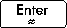
\includegraphics{HPPrime-Enter.pdf} \textsfs{(0,0.1)} 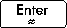
\includegraphics{HPPrime-Enter.pdf} \textsfs{(0.6,0.45)} 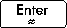
\includegraphics{HPPrime-Enter.pdf}, i  escrivim després el nom del programa: \textsfs{EZS\_U()}.

        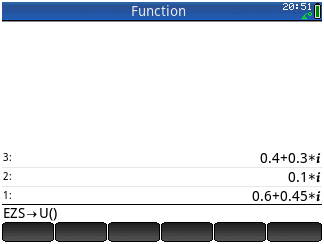
\includegraphics{Cap-CalcBas-EZS-HPP1.png}

    \item Premem a continuació la tecla 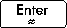
\includegraphics{HPPrime-Enter.pdf} i la calculadora ens dona el valor de la tensió $\cmplx{U}$.

        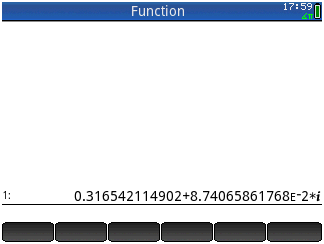
\includegraphics{Cap-CalcBas-EZS-HPP2.png}


     \item   Si la calculadora estigués en el mode \textsfs{Algebraic} o en el mode  \textsfs{Textbook}, escriuríem directament: \textsfs{EZS\_U(0.4+0.3*}\textit{\textbf{i}}, \textsfs{0.1*}\textit{\textbf{i}}, \textsfs{0.6+0.45*}\textit{\textbf{i}}\textsfs{)}, i després de prémer la tecla 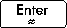
\includegraphics{HPPrime-Enter.pdf} la calculadora ens donaria el valor de la tensió $\cmplx{U}$.

        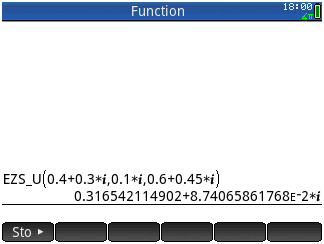
\includegraphics{Cap-CalcBas-EZS-HPP3.png}

    \end{dingautolist}
\end{exemple}



\section{Corrent de curtcircuit en el  secundari d'un transformador}
\index{corrent!de curtcircuit!en el  secundari d'un transformador}\label{sec:cc-sec-trafo}

 Es tracta en aquest apartat el càlcul del corrent de curtcircuit trifàsic en el secundari d'un transformador que té el
primari connectat  a una xarxa de potència.

A partir de la figura \vref{pic:cc_sec_trafo}, es tracta de trobar
el valor del corrent de curtcircuit trifàsic $I\ped{F}$ en el punt
F, essent coneguts la resta de paràmetres.

\begin{center}
    \input{Imatges/Cap-CalcBas-Icc-Trafo.pdf_tex}
    \captionsetup{justification=raggedright,margin={4cm,4cm},oneside}
    \captionof{figure}{Corrent de curtcircuit en el  secundari d'un transformador} \label{pic:cc_sec_trafo}
\end{center}

$U$, $U\ped{T1}$ i $U\ped{T2}$ estan donats en volt,
$S\ped{cc}$ i $S\ped{T}$ en voltampere, i $x\ped{cc}$ en tant per u
respecte dels valors nominals del transformador.


Per tal de simplificar el problema, suposarem que tant la impedància
de curtcircuit del transformador com la impedància equivalent de
la xarxa de potència són totalment inductives; d'aquesta manera
podrem treballar amb les diverses variables implicades com si
fossin nombres reals. Suposarem a més que no hi ha circulació de
corrent abans del curtcircuit.

Pel que fa a la xarxa de potència, si en lloc de la potència de curtcircuit $S\ped{cc}$, el que coneixem és el corrent de curtcircuit
disponible $I\ped{cc}$, podem obtenir el valor de la potència de
curtcircuit a partir de l'expressió:
\begin{equation}
    S\ped{cc} = \sqrt{3} U I\ped{cc}
\end{equation}
\index{potència!de curtcircuit}

 Si prenem com a valors base els
paràmetres del transformador ($U\ped{T1}$, $U\ped{T2}$ i
$S\ped{T}$), la relació de transformació i la impedància de curtcircuit del transformador, expressats en tant per u, seran 1:1 i
$x\ped{cc}$ respectivament. Anàlogament, la tensió i la impedància
equivalents de la xarxa de potència, expressats en tant per u, seran
$\frac{U}{U\ped{T1}}$ i $\frac{U^2}{S\ped{cc}}
\frac{S\ped{T}}{U\ped{T1}^2}$ respectivament.

El corrent de curtcircuit és igual a la tensió en el punt F prèvia al curtcircuit, dividida per la impedància vista des d'aquest punt (vegeu la secció \ref{sec:xarxes-curtcircuits}). Expressat en tant per u, el corrent de curtcircuit $i\ped{F}$ és:

\begin{equation}
    i\ped{F} = \frac{\dfrac{U}{U\ped{T1}}}{\dfrac{U^2}{S\ped{cc}}
    \dfrac{S\ped{T}}{U\ped{T1}^2} + x\ped{cc}}
\end{equation}

En conseqüència, aquest corrent $I\ped{F}$ expressat en ampere val:

\begin{equation}
    I\ped{F} = i\ped{F}\; \frac{S\ped{T}}{\sqrt{3}U\ped{T2}} =
    \frac{S\ped{T} U}{\sqrt{3} U\ped{T1}U\ped{T2}
    \left(\dfrac{U^2}{S\ped{cc}}
    \dfrac{S\ped{T}}{U\ped{T1}^2} + x\ped{cc}\right)}
\end{equation}

Si la xarxa de potència es considera de potència infinita, tenim:

\begin{equation}
    I\ped{F} = \frac{S\ped{T} U}{\sqrt{3} U\ped{T1}U\ped{T2}
    x\ped{cc}},\qquad \text{amb }S\ped{cc}=\infty
\end{equation}

Si  la tensió de la xarxa coincideix amb la tensió primària
del transformador, tenim respectivament:
\begin{align}
    I\ped{F} &= \frac{S\ped{T}}{\sqrt{3} U\ped{T2}
    \left(\dfrac{S\ped{T}}{S\ped{cc}} +
    x\ped{cc}\right)},\qquad \text{amb }U=U\ped{T1}\\[1ex]
    I\ped{F} &= \frac{S\ped{T}}{\sqrt{3} U\ped{T2}
    x\ped{cc}}, \qquad \text{amb }U=U\ped{T1}\text{ i }
    S\ped{cc}=\infty
\end{align}


\begin{exemple}[\CorrentCcSecTrafo{}]
	\addcontentsxms{\CorrentCcSecTrafo}
    A partir de la figura \vref{pic:cc_sec_trafo}, amb els valors
    $U=\qty{6900}{V}$, $U\ped{T1}=\qty{6900}{V}$,
    $U\ped{T2}=\qty{400}{V}$, $S\ped{T}=\qty{850}{kVA}$ i
    $x\ped{cc}=\qty{5}{\percent}$, es tracta de trobar $I\ped{F}$ en el cas
    que: a) $S\ped{cc}=\qty{200}{MVA}$, i b) $S\ped{cc}=\infty$.

    Els valors demanats són:
    \begin{align*}
       &a)\;I\ped{F} = \frac{\qty{850}{kVA}}{\sqrt{3}\times \qty{400}{V}\times
       \left(\dfrac{\qty{850}{kVA}}{\qty{200}{MVA}} +
       \num{0,05}\right)} = \qty{22,6}{kA} \\[2ex]
       &b)\;I\ped{F} = \frac{\qty{850}{kVA}}{\sqrt{3}\times \qty{400}{V}\times
       \num{0,05}} = \qty{24,5}{kA}
    \end{align*}

\end{exemple}



\section{Escales logarítmiques}\label{sec:escales-log} \index{escales logarítmiques}

\subsection{Determinació de punts d'una corba}\index{escales logarítmiques!determinació de punts d'una corba}

En diferents camps de l'electrotècnia és usual trobar gràfics amb escales
logarítmiques.

Un exemple clar són els gràfics d'actuació dels interruptors magnetotèrmics o dels
fusibles, on les seves corbes característiques corrent-temps estan representades en
una escala logarítmica-logarítmica o lineal-logarítmica.

En aquests casos es presenta sovint la necessitat de determinar amb exactitud un
punt de la corba que no coincideix amb cap de les línies divisòries del gràfic. Atesa
la figura \vref{pic:escala log}, es tractaria de determinar el valor $x$ dins de la dècada
$10^N$ a $10^{N+1}$.

\begin{center}
    \input{Imatges/Cap-CalcBas-EscalesLog.pdf_tex}
    \captionof{figure}{Escala logarítmica}
    \label{pic:escala log}
\end{center}

Si mesurem amb un regle la distància $D$ des de l'inici de la dècada fins al punt $x$, i
la longitud total $L$ de la dècada, el valor $x$ buscat és definit per l'expressió:

\begin{equation}
    x = 10^{\left(N+\frac{D}{L}\right)}
\end{equation}

Si estem interessats en el problema invers, és a dir, en  trobar la distància $D$
corresponent a un valor conegut $x$ dins de la dècada $10^N$ a $10^{N+1}$, podem emprar
l'expressió:

\begin{equation}
    D = L(\log x - N) = L \log\frac{x}{10^N}
\end{equation}

	
\begin{exemple}[\ValorsEscalaLog{}]
	\addcontentsxms{\ValorsEscalaLog}
    Es tracta de trobar, en primer lloc, el valor $x$ dins de la dècada 100 a 1000, corresponent a una
    distància $D=\qty{11}{mm}$, i, en segon lloc, la distància $D$ a la qual hem de representar el valor $x=5$, dins de la
    dècada 1 a 10. La longitud total d'una dècada és $L=\qty{56}{mm}$.

    En el primer cas tenim $N=2$; en conseqüència:
    \[
        x = 10^{\left(2+\frac{\qty{11}{mm}}{\qty{56}{mm}}\right)}= \num{157,19}
    \]

    En el segon cas tenim $N=0$; en conseqüència:
    \[
        D = \qty{56}{mm} \times (\log 5 - 0)  = \qty{39,1}{mm}
    \]

\end{exemple}

\subsection{Determinació dels paràmetres d'una funció representada com una recta}\label{sec:escales-log-yxnk}\index{escales logarítmiques!determinació dels paràmetres d'una funció representada com una recta}

Quan la relació entre dues variables $y=f(x)$ compleix l'equació: $y x^n = k$, on $n$ i $k$  són constants  reals, la gràfica d'aquesta funció pren la forma d'una línia recta quan es representa en una escala logarítmica-logarítmica. Partint de l'equació inicial $y x^n = k$, si passem la variable $x$ a la dreta, tenim:
\begin{equation}
  y = k x^{-n}
\end{equation}

Prenent logaritmes a banda i banda, tenim:
\begin{equation}
  \log y = \log k - n \log x
\end{equation}

Aquesta és l'equació d'una recta de pendent negatiu $n$, amb les variables $\log y$ i $\log x$.

A partir de la gràfica d'una recta en una escala logarítmica-logarítmica, podem determinar-ne les constants $n$ i $k$ seguint els passos següents:

\begin{dingautolist}{202}
    \item Per  determinar el pendent $n$, només cal mesurar directament sobre la gràfica amb un regle, una distància horitzontal $\Delta{}x$ i una de vertical $\Delta{}y$ que partint d'un punt de la recta ens portin a un altre punt de la mateixa recta; a partir d'aquests dos valors, tenim:
        \begin{equation}
          n = \frac{\Delta{}y}{\Delta{}x}
        \end{equation}

        Aquesta equació suposa que la gràfica té una relació d'aspecte  1:1, és a dir, que una dècada vertical i una d'horitzontal tenen la mateixa llargada. Si, per exemple, les dècades verticals tinguessin la meitat de la llargada que les dècades  horitzontals, caldria multiplicar per dos el valor mesurat de $\Delta{}y$.

   \item  Un cop  coneixem $n$, a partir d'un punt qualsevol $(x_1, y_1)$ de la recta, podem calcular $k$ utilitzant l'equació inicial $y x^n = k$:
        \begin{equation}
          k =  y_1 x_1^n
        \end{equation}

        En el cas particular de $x_1=1$, l'equació anterior se simplifica a:\begin{equation}
           k = y_1, \quad \text{amb }x_1=1
        \end{equation}
\end{dingautolist}

Aquest tipus de relació es compleix, per exemple, en el cas dels cables elèctrics, entre el corrent de curtcircuit i el temps que el cable pot aguantar aquest corrent sense malmetre's. Vegeu la secció \vref{ces:cables_Icc_termica}.

	
\begin{exemple}[\ConstantsEscalaLogLog{}]
	\addcontentsxms{\ConstantsEscalaLogLog}
    Es tracta de trobar les constants $n$ i $k$ de la funció que apareix dibuixada com una recta en la gràfica de la pàgina següent.

     Atès que la gràfica té una relació d'aspecte 1:1, a partir dels valors mesurats $\Delta{}y$ i $\Delta{}x$, tenim:
    \[
        n = \frac{\qty{171,6}{mm}}{\qty{57,2}{mm}} = 3
    \]

    Partint, per exemple, del valor d'abscisses $x_1=100$, veiem que el valor corresponent d'ordenades és: $y_1=2$;  per tant, tenim:
    \[
        k = 2 \times 100^3  = \num{2000000}
    \]

    L'equació que segueix aquesta funció, és doncs:
    \[
        y x^3 = \num{2000000}
    \]

   \begin{center}
        % GNUPLOT: LaTeX picture with Postscript
\begingroup
  \makeatletter
  \providecommand\color[2][]{%
    \GenericError{(gnuplot) \space\space\space\@spaces}{%
      Package color not loaded in conjunction with
      terminal option `colourtext'%
    }{See the gnuplot documentation for explanation.%
    }{Either use 'blacktext' in gnuplot or load the package
      color.sty in LaTeX.}%
    \renewcommand\color[2][]{}%
  }%
  \providecommand\includegraphics[2][]{%
    \GenericError{(gnuplot) \space\space\space\@spaces}{%
      Package graphicx or graphics not loaded%
    }{See the gnuplot documentation for explanation.%
    }{The gnuplot epslatex terminal needs graphicx.sty or graphics.sty.}%
    \renewcommand\includegraphics[2][]{}%
  }%
  \providecommand\rotatebox[2]{#2}%
  \@ifundefined{ifGPcolor}{%
    \newif\ifGPcolor
    \GPcolortrue
  }{}%
  \@ifundefined{ifGPblacktext}{%
    \newif\ifGPblacktext
    \GPblacktexttrue
  }{}%
  % define a \g@addto@macro without @ in the name:
  \let\gplgaddtomacro\g@addto@macro
  % define empty templates for all commands taking text:
  \gdef\gplbacktext{}%
  \gdef\gplfronttext{}%
  \makeatother
  \ifGPblacktext
    % no textcolor at all
    \def\colorrgb#1{}%
    \def\colorgray#1{}%
  \else
    % gray or color?
    \ifGPcolor
      \def\colorrgb#1{\color[rgb]{#1}}%
      \def\colorgray#1{\color[gray]{#1}}%
      \expandafter\def\csname LTw\endcsname{\color{white}}%
      \expandafter\def\csname LTb\endcsname{\color{black}}%
      \expandafter\def\csname LTa\endcsname{\color{black}}%
      \expandafter\def\csname LT0\endcsname{\color[rgb]{1,0,0}}%
      \expandafter\def\csname LT1\endcsname{\color[rgb]{0,1,0}}%
      \expandafter\def\csname LT2\endcsname{\color[rgb]{0,0,1}}%
      \expandafter\def\csname LT3\endcsname{\color[rgb]{1,0,1}}%
      \expandafter\def\csname LT4\endcsname{\color[rgb]{0,1,1}}%
      \expandafter\def\csname LT5\endcsname{\color[rgb]{1,1,0}}%
      \expandafter\def\csname LT6\endcsname{\color[rgb]{0,0,0}}%
      \expandafter\def\csname LT7\endcsname{\color[rgb]{1,0.3,0}}%
      \expandafter\def\csname LT8\endcsname{\color[rgb]{0.5,0.5,0.5}}%
    \else
      % gray
      \def\colorrgb#1{\color{black}}%
      \def\colorgray#1{\color[gray]{#1}}%
      \expandafter\def\csname LTw\endcsname{\color{white}}%
      \expandafter\def\csname LTb\endcsname{\color{black}}%
      \expandafter\def\csname LTa\endcsname{\color{black}}%
      \expandafter\def\csname LT0\endcsname{\color{black}}%
      \expandafter\def\csname LT1\endcsname{\color{black}}%
      \expandafter\def\csname LT2\endcsname{\color{black}}%
      \expandafter\def\csname LT3\endcsname{\color{black}}%
      \expandafter\def\csname LT4\endcsname{\color{black}}%
      \expandafter\def\csname LT5\endcsname{\color{black}}%
      \expandafter\def\csname LT6\endcsname{\color{black}}%
      \expandafter\def\csname LT7\endcsname{\color{black}}%
      \expandafter\def\csname LT8\endcsname{\color{black}}%
    \fi
  \fi
    \setlength{\unitlength}{0.0500bp}%
    \ifx\gptboxheight\undefined%
      \newlength{\gptboxheight}%
      \newlength{\gptboxwidth}%
      \newsavebox{\gptboxtext}%
    \fi%
    \setlength{\fboxrule}{0.5pt}%
    \setlength{\fboxsep}{1pt}%
    \definecolor{tbcol}{rgb}{1,1,1}%
\begin{picture}(9060.00,12740.00)%
    \gplgaddtomacro\gplbacktext{%
      \colorrgb{0.00,0.00,0.00}%%
      \put(816,900){\makebox(0,0)[r]{\strut{} 0,1}}%
      \colorrgb{0.00,0.00,0.00}%%
      \put(816,4724){\makebox(0,0)[r]{\strut{} 1}}%
      \colorrgb{0.00,0.00,0.00}%%
      \put(816,8547){\makebox(0,0)[r]{\strut{} 10}}%
      \colorrgb{0.00,0.00,0.00}%%
      \put(816,12371){\makebox(0,0)[r]{\strut{} 100}}%
      \colorrgb{0.00,0.00,0.00}%%
      \put(997,603){\makebox(0,0){\strut{} 10}}%
      \colorrgb{0.00,0.00,0.00}%%
      \put(4821,603){\makebox(0,0){\strut{} 100}}%
      \colorrgb{0.00,0.00,0.00}%%
      \put(8645,603){\makebox(0,0){\strut{} 1000}}%
      \csname LTb\endcsname%%
      \put(824,5875){\makebox(0,0)[r]{\strut{}2}}%
    }%
    \gplgaddtomacro\gplfronttext{%
      \csname LTb\endcsname%%
      \put(504,6636){\makebox(0,0){\strut{}$y$}}%
      \csname LTb\endcsname%%
      \put(8698,6636){\rotatebox{-270}{\makebox(0,0){\strut{}}}}%
      \csname LTb\endcsname%%
      \put(4821,284){\makebox(0,0){\strut{}$x$}}%
      \csname LTb\endcsname%%
      \put(4821,12371){\makebox(0,0){\strut{}}}%
      \csname LTb\endcsname%%
      \put(2647,7221){\rotatebox{-270}{\makebox(0,0){\strut{}$\Delta{}y =\qty{171,6}{mm}$}}}%
      \csname LTb\endcsname%%
      \put(3973,2171){\makebox(0,0){\strut{}$\Delta{}x =\qty{57,2}{mm}$}}%
      \csname LTb\endcsname%%
      \put(4821,12371){\makebox(0,0){\strut{}}}%
    }%
    \gplbacktext
    \put(0,0){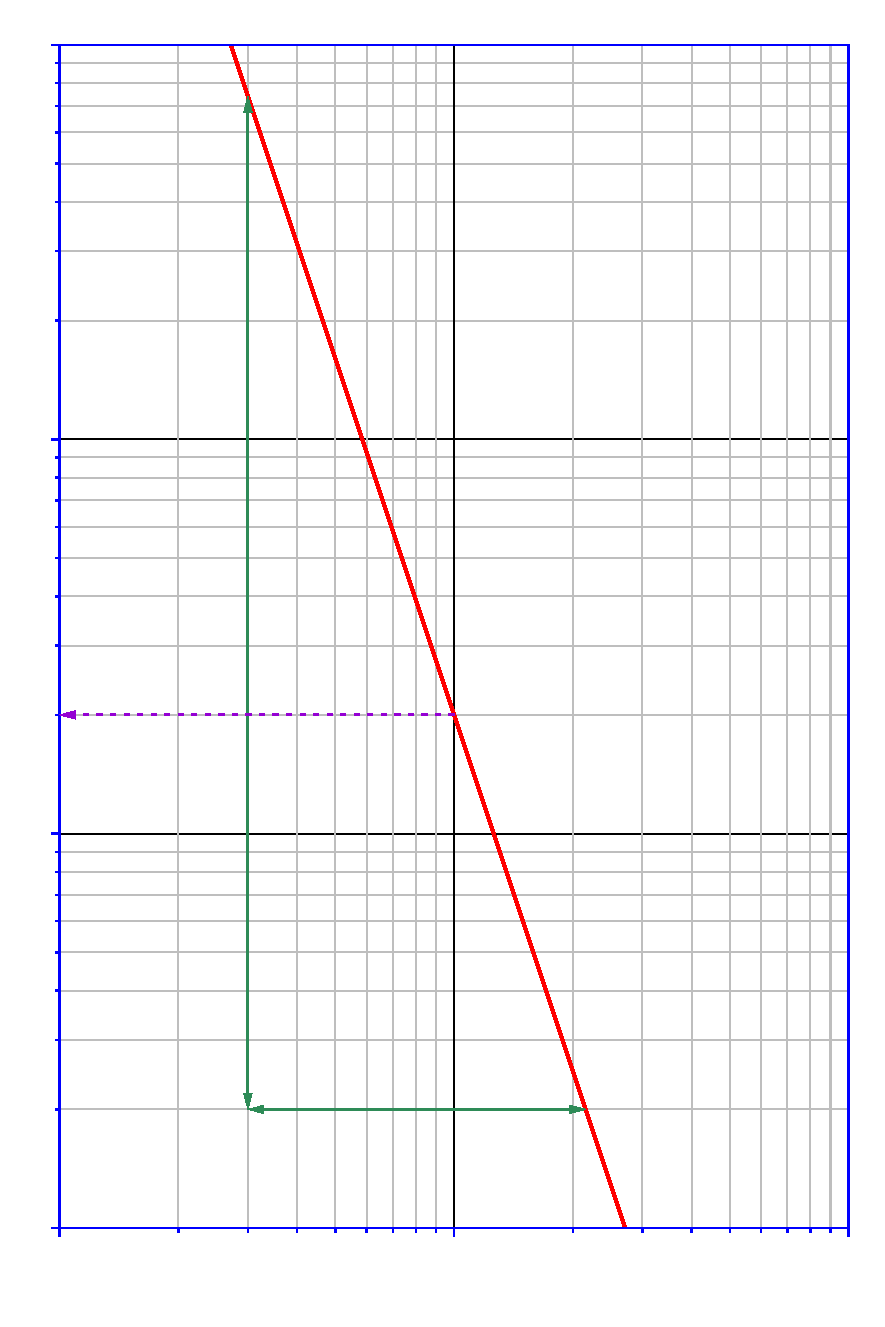
\includegraphics[width={453.00bp},height={637.00bp}]{Cap-CalcBas-RectaLogLog}}%
    \gplfronttext
  \end{picture}%
\endgroup

   \end{center}

\end{exemple}

